\chapter{IGT2P: From Interlinear Glossed Texts to Paradigms}
\label{chap:IGT2P}


%The paradigms allow linguists to learn, generalized, and describe inflection patterns and inflection classes. 
The typical next step in the language documentation and description workflow following morpheme segmentation and glossing is finding and organizing inflected forms that are attested in the transcribed natural speech. Then, because full paradigms rarely occur in natural speech, complete morphological paradigms are elicited. This can be done by using the inflected forms found in IGT to hypothesize and generate new inflected forms that might complete a lexeme's inflectional paradigm. This chapter describes a task that can speed this process and automatically generate the ``missing'' morphological forms.

This task, which we call \textbf{IGT-to-paradigms}\footnote{IGT2P was introduced as a new task by \citet{moeller_igt2p_2020}} (IGT2P), differs from the existing \textit{morphological inflection} \citep{yarowsky-wicentowski-2000-minimally,faruqui-etal-2016-morphological} task in three aspects: (1) inflected forms extracted from IGT are noisier than curated training data for morphological generation, (2) since lemmas are not explicitly identified in IGT, systems cannot be trained on typical lemma-to-form mappings and, instead, must be trained on form-to-form mappings, and (3) part-of-speech (POS) tags are often unavailable in IGT. IGT2P can thus be seen as a noisy version of morphological \textit{re}inflection \citep{cotterell-etal-2016-sigmorphon}, but without explicit POS information. Our experiments show that after preprocessing the data existing morphological reinflection systems are strong baselines for this task. 

IGT2P generates entire morphological paradigms from IGT input and can be used to generate new morphological resources for natural language processing systems in low-resource settings. NLP systems that account for morphology can reduce data sparsity caused by an abundance of individual word forms in morphologically rich languages \citep{cotterell-etal-2016-sigmorphon,cotterell-etal-2017-conll,cotterell-etal-2018-conll,mccarthy-etal-2019-sigmorphon,vylomova2020sigmorphon} and help mitigate bias in training data for natural language processing (NLP) systems \citep{zmigrod-etal-2019-counterfactual}. Over the last few years, multiple shared tasks have encouraged the development of systems for learning morphology, including those that generate inflected forms of the canonical form, or lemma, of a lexeme.  However, such systems have often been limited to languages with publicly available structured data, i.e., languages for which complete tables containing inflectional paradigmatic information can be found, for example, in Wiktionary.\footnote{\url{https://www.wiktionary.org}} This limits the development of NLP systems for morphology to those languages for which morphological information can be easily extracted. 

IGT2P instead makes use of a resource which is much more common, especially for low-resource languages:
we explore how to leverage interlinear glossed text (IGT) to generate unseen forms of inflectional paradigms, as illustrated in Figure \ref{fig:Workflow}. Field IGT has not been used in NLP for various reasons. One reason is the nature of the data itself which is discussed in \ref{sec:issues}. Another reason is the difficulty of bringing the data to the state found in resources such as Wiktionary or Unimorph.\footnote{\url{https://www.unimorph.org}} This chapter explores whether having a language expert spend only a few hours cleaning the noisy IGT data improves the task's performance. 


% flowchart IGT to paradigm completion
\begin{figure}[!tb]
    \centering
    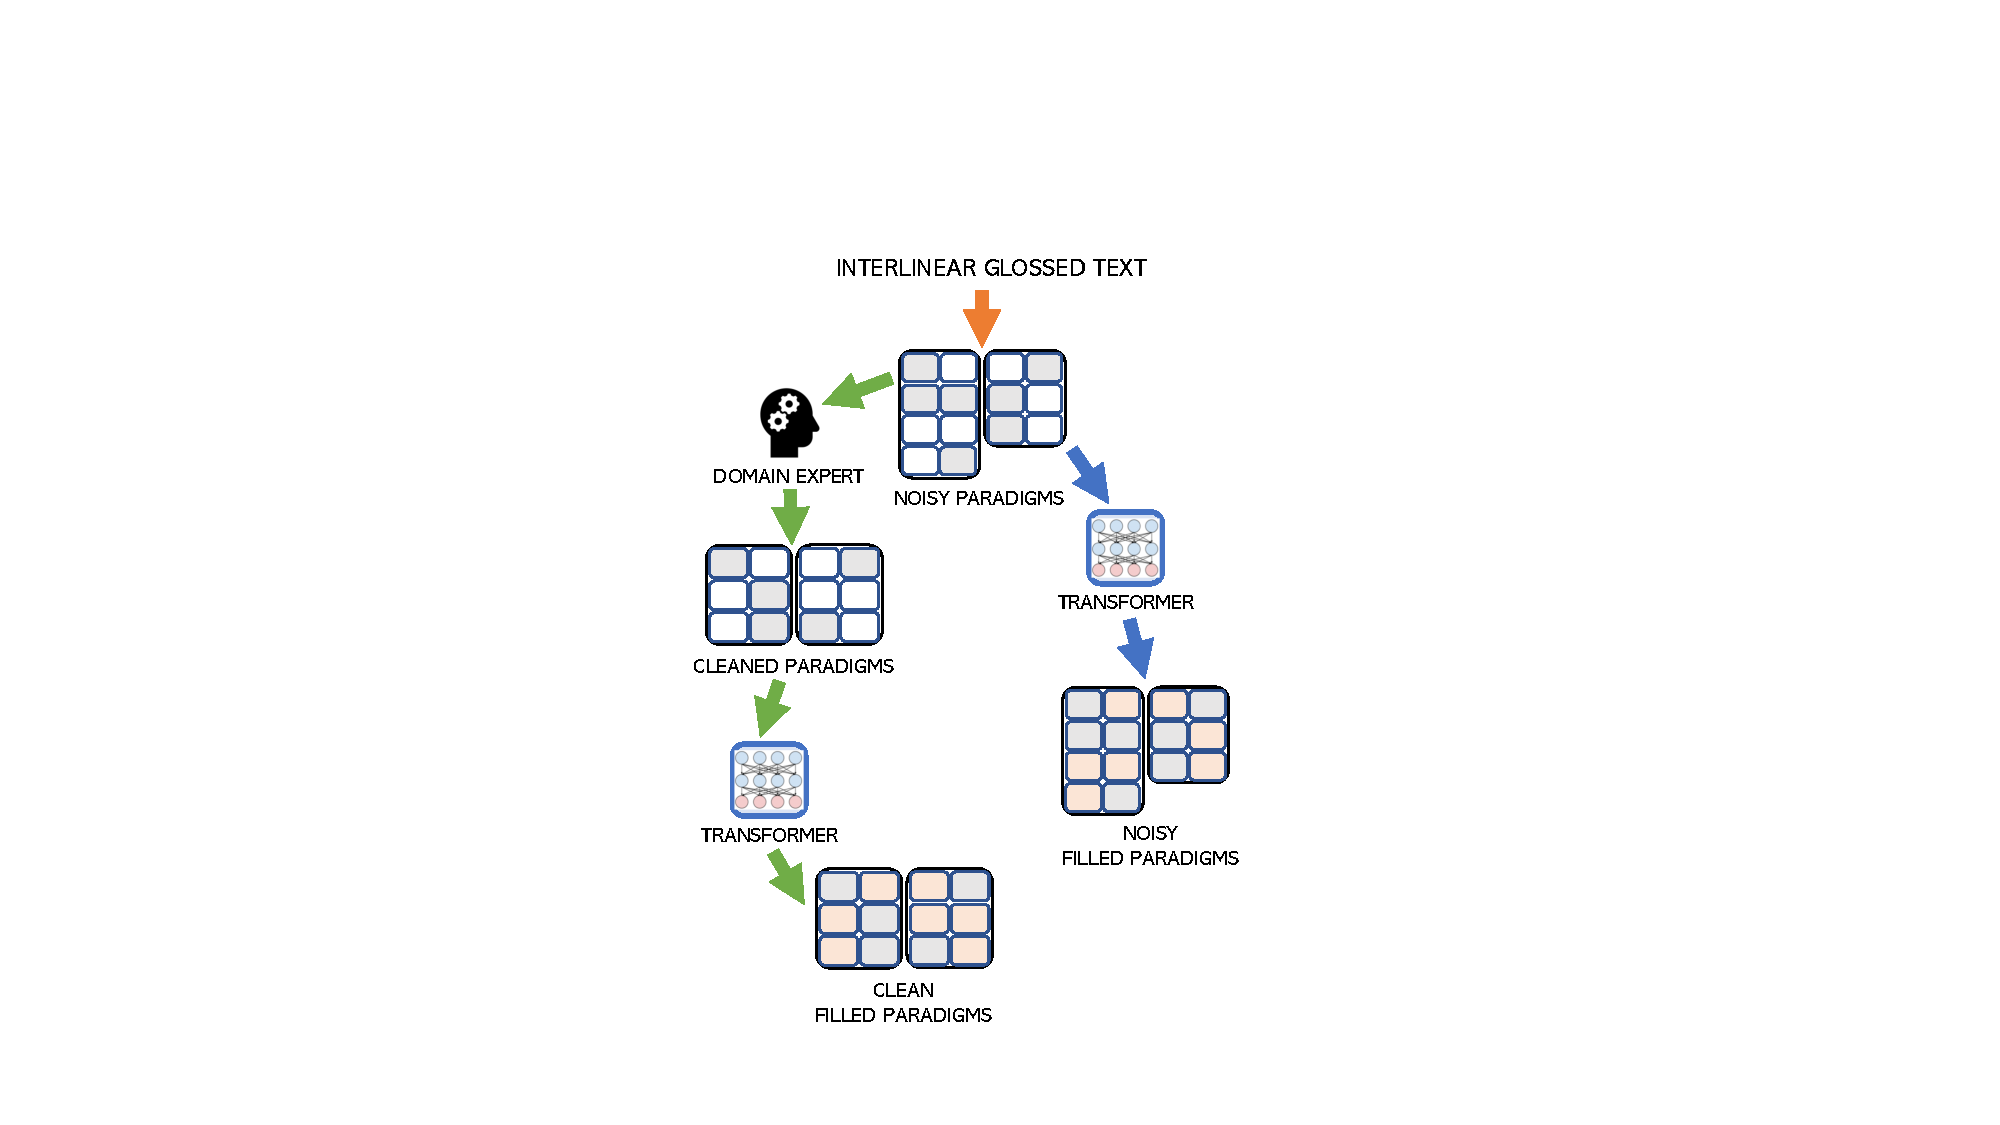
\includegraphics[width=8cm]{figs/IGT-Paradigm-Workflow2.pdf}
    \caption[IGT2P Overview]{Inflected word forms attested in interlinear glossed texts (IGT) train Transformer encoder-decoder to generalize morphological paradigmatic patterns and generate word forms when given known morphosyntatic features of missing paradigm cells. Noisy paradigms are automatically constructed from IGT and a language expert creates ``cleaned'' paradigms. Both sets are tested on the same missing word forms and the results are compared.}
    \label{fig:Workflow}
\end{figure}


Thus, this chapter asks two related questions: 
\begin{itemize}
    \item To what extent can manually interlinearized texts be utilized for computational induction of morphological inflection paradigms? 
    \item How much does manual cleaning of IGT data by a domain expert improve performance?
\end{itemize}

The first question is answered using existing morphological reinflection models and documentary and descriptive data and the IGT2P task. IGT2P can successfully induce morphological paradigms with $21\%$ to $64\%$ accuracy. The second question is answered by examining which inflection model performs better on noisy and cleaned IGT data. Cleaning the data improves performance across the board with a Transformer by $1.27\%$ to $16.32\%$. 


\section{IGT-to-Paradigms (IGT2P)}

The task presented here, IGT-to-paradigms (IGT2P), can be described formally as the paradigm completion problem described in Chapter \ref{chap:litreview}, with an additional step of inference regarding which of the attested forms is associated with which lemma. 

Formally, during training the systems are given a list of input words with -- potentially empty -- morphological feature vectors $\mathcal{D}=(w_1,\vec{t}_1) \dots, (w_{|\mathcal{D}|}, \vec{t}_{|\mathcal{D}|})$ and a list $\mathcal{U} = \{u_j\}$ of $|\mathcal{U}|$~inflected words, $u_j = f(\ell_j, \vec{t}_{\gamma_j})$. The goal of IGT2P is to generate the paradigms 
$\{\pi(\ell_j)\}_{f(\ell_j, \vec{t}_{\gamma_j})\in\mathcal{U}}$ from the information available in IGT. This method is illustrated in \autoref{fig:IGT2P}.

\begin{figure}[!tb]
    \centering
    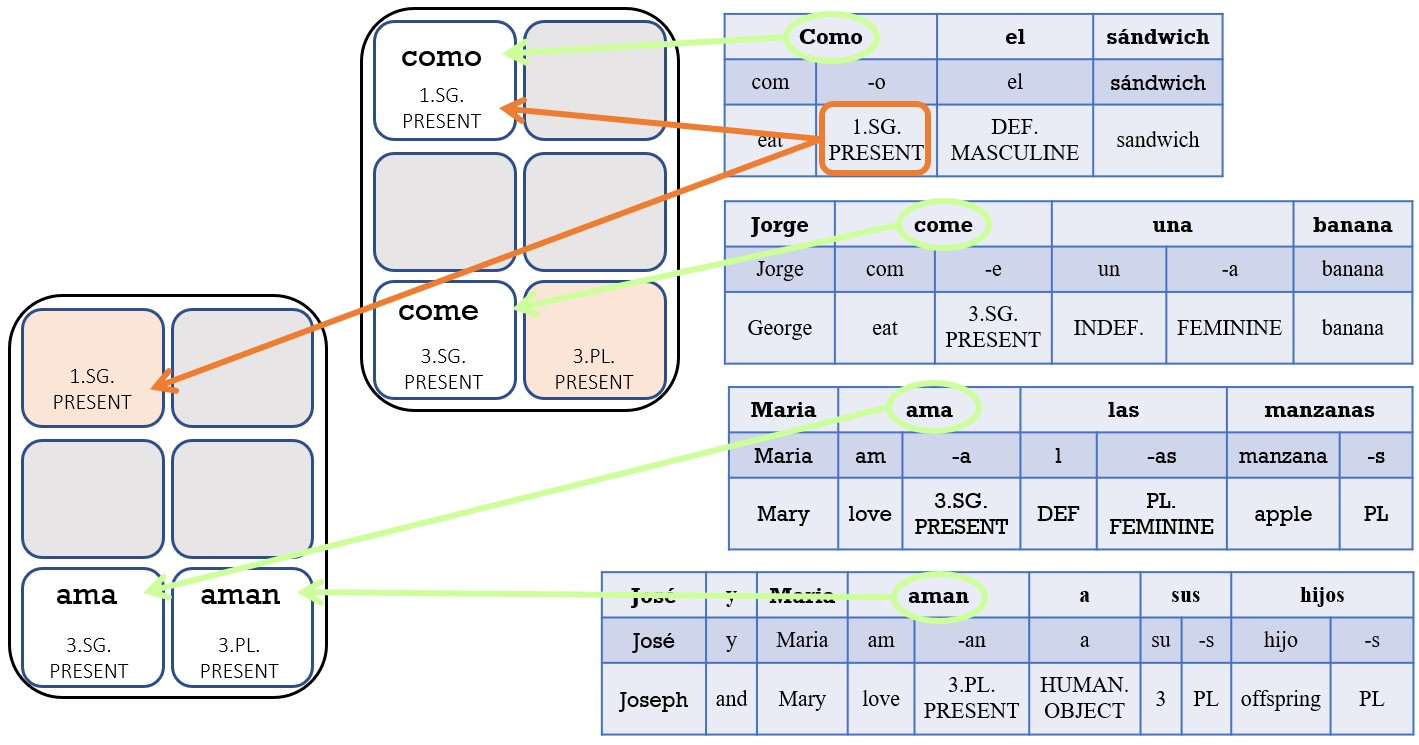
\includegraphics[width=16cm]{figs/IGT2P.jpg}
    \caption[IGT2P]{IGT2P learns inflectional paradigms by filling paradigm table cells with inflected forms attested in IGT data such as this mini-Spanish corpus gathered from fluent speakers. The grayed cells represent forms that are not attested in the mini IGT corpus and can only be hypothesized to exist in the language. The orange cells also represent forms not attested in the data, but they are known to exist because of the morphosyntactic features of the cell are attested by other lemmas (i.e., \textit{como} `I eat'). A machine learning model predicts the missing forms (i.e., \textit{amo} `I love' and \textit{comen} `they eat') of the orange cells. In documentary and descriptive fieldwork, the predicted forms can serve as a hypothesis that linguists can use to help elicit further information about the language's inflectional patterns.}
    \label{fig:my_label}
\end{figure}

Like unsupervised paradigm completion, IGT2P does not assume information about the lemma to be explicit. Like morphological reinflection, the input includes word forms with features, and a system must learn to generate inflections from other word forms and morphological feature vectors. 
%Although While it is not clear or enforced that more than one form is given for any paradigm, 
IGT2P is further like paradigm completion in that it aims at generating \textit{all} inflected forms for each lemma.\footnote{Currently this is approximated during evaluation, since gold standard paradigms do not exist for all the languages/dialects. Also, the list $\mathcal{U}$ consists of words in $\mathcal{D}$ but we do not include those in the input so that the words in $\mathcal{D}$ have not been seen by the model.} Instead of generating paradigms from raw text, IGT2P generates them from IGT, a resource available for many under-studied languages.


\section{Why IGT2P?}

\begin{table}[tb]
    \centering
    \begin{tabular}{rlllll}
       \textbf{Text}  & Vecherom & ya & pobejala & v & magazin. \\
      \textbf{Segmented}   & vecher-om & ya & pobeja-la & v & magazin \\
      \textbf{Glossed} & evening-\textsc{ins} & \textsc{1.sg.nom} & run-\textsc{pfv.pst.sg.fem} & in & store.\textsc{acc} \\
      \textbf{Translation} & \multicolumn{5}{l}{`In the evening I ran to the store.'}
    \end{tabular}
    \caption[IGT example]{An example of typical interlinear glossed text (IGT) with a transliterated Russian sentence, including translation. IGT2P leverages the original text and gloss lines.}
    \label{tab:IGT}
\end{table}


Descriptive linguistics aims to objectively analyze primary language data in new languages and publish descriptions of their structure. This work informs our understanding of human language and provides resources for NLP development through academic literature, which informs projects such as UniMorph \citep{kirov_unimorph}, or through crowdsourced efforts such as Wiktionary. Yet since most descriptive work is performed manually with minimal, if any, NLP assistance, language resources for thousands of under-described languages remain limited. This includes languages with millions of speakers, such as Manipuri in India.

However, there exists a type of labeled data that is available in nearly all languages that a linguist has documented or described: \textit{interlinear glossed texts} (IGT), illustrated in Table \ref{tab:IGT}. They are the output of early steps in a field linguist's pipeline which consist of recording natural speech, transcribing it, and then identifying minimal meaningful units---the morphemes---and using internally consistent tags to label the morphemes' morphosyntactic features. IGTs serve as vital sources of morphological, syntactic, and higher levels of linguistic information. They are often archived in long-term repositories, and openly accessible for non-commercial purposes, yet they are rarely utilized in NLP.

IGT2P has potential benefits for NLP (by increasing available resources in low-resource languages) but also for linguistic inquiry. First, since machine-assistance has been shown to increase speed and accuracy of manual linguistic annotation with just 60\% model accuracy \citep{felt_improving_2012}, such a model could assist the initial analysis of morphological patterns in IGT. Second, by quickly learning morphological patterns from word forms attested in IGT, IGT2P generates forms that fill empty cells in a lemma's paradigm. Since IGTs are unlikely to contain complete paradigms of lemmas, an accompanying step in fieldwork is that of elicitation of inflectional paradigms for selected lemmas. Presenting candidate words to a native speaker for acceptance or rejection is often easier than asking the speaker to grasp the abstract concept of a paradigm and to generate the missing cells in a table. With the help of IGT2P, linguists could use the machine-generated word forms to support this elicitation process. IGT2P then becomes a tool for the discovery of morphological patterns in under-described and endangered languages.



\section{Issues specific to IGT}
\label{sec:issues}

The most notable issue with IGT is the ``noise''. An inevitable cause is the dynamic nature of ongoing linguistic analysis. As the linguist gains a better understanding of the language's structure by doing interlinearization, early decisions about morpheme shapes and glosses differ from later ones. Another cause is that limited budget and time means IGT are often only partially completed. Another source of noise comes when the project is focused on annotating one particular phenomenon. For example, frequently only one morphosyntactic feature in Manipuri was glossed in each word, meaning different inflected forms looked like they had the same morphosyntactic features. Another source of noise is imprecision introduced by human errors or choices made for convenience to speed tedious annotation. One example of imprecision is glossing different stem morphemes with the same English word. For example, Lezgi has several copula verbs which can be narrowly translated as `be in', `be at', etc., but most were merely glossed as `be'. So, all copula verbs were initially grouped into one paradigm. An analogous situation happened with Arapaho: nuances of meaning were not often distinguished in the glosses; thus, different verb stems are glossed simply as ‘give’, when they should be divided into ‘hand to someone’ in one case, ‘give as a present’ in another case, and ‘give ceremonially, as an honor’ in third case.
%Moreover, they do not make a difference between stems linking inanimate subjects and animate subjects. 

Another issue is that IGT annotators do not usually differentiate between distinct types of morphemes. Thus, we do not always distinguish them. Derivational and inflectional morphemes were only differentiated where we were able to easily identify and eliminate derivational glosses. For example, in Arapaho we were able to group derived stems into separate paradigms because they were glossed distinctly. Also, clitics are often not distinguished from affixes. This means that the morphological patterns that the models learn are not always, strictly speaking, inflectional paradigms, but it does mean that the models learn all attested forms related to one lemma.
%, to the extent these forms are attested in the annotations and their stems glossed identically.


\section{Experimental Approach}

From the IGT corpora described in Chapter \ref{chap:datamodels} this study used Arapaho, Alas, Lezgi, Manipuri, Nat\"ugu, and Tsez.
As a first step, partial inflectional paradigms were automatically extracted from the IGT. Words were organized into paradigms based on the gloss of the stem morpheme. Then, these stem glosses were removed, leaving only the affix glosses which serve as morphosyntactic feature tags. The data is summarized in Table \ref{tab:IGT2Pdata}.

\begin{table}[!tb]
    \centering
    %\setlength{\tabcolsep}{5.pt}
    \begin{tabular}{l|ccccccc}
       \textbf{Language} & \textbf{paradigms} & \textbf{single-entry} & \textbf{tokens} & \textbf{train} & \textbf{dev} & \textbf{test} & \textbf{unannot}  \\
       \hline
       arp clean & 16,857 & 10,857 & 56,644 & 283,714 & \multirow{2}{*}{14,151} & \multirow{2}{*}{14,150} & \multirow{2}{*}{6,877} \\
       arp noisy & 14,389 & 8,855 & 56,922 & 435,430 & & &  \\
       % single to multi entry proportion: .644
       % unannotated to total words proportion: .121
       %& 14,151  \\
       \hline
       btz clean & 247 & 172 & 386 & 354 & \multirow{2}{*}{52}  & \multirow{2}{*}{52} & \multirow{2}{*}{1,106} \\
       btz noisy & 235 & 150 & 412 & 575 & & & \\
       \hline
       ddo clean & 982 & 330 & 7,221 & 35,773 & \multirow{2}{*}{2,173} & \multirow{2}{*}{2,172} & \multirow{2}{*}{9,408} \\
       ddo noisy & 945 & 295 & 7,315 & 36,875 & & &  \\
       % single to multi entry proportion: .305
       % unannotated to total words proportion: 1.302
       \hline
       lez clean & 301 & 202 & 543 & 539 & \multirow{2}{*}{88} & \multirow{2}{*}{88} & \multirow{2}{*}{3,054} \\
       lez noisy & 298 & 188 & 588 & 1,254 &  &  &  \\
       % single to multi entry proportion: .671
       % unannotated to total words proportion: 5.624
       \hline
       mni clean & 479 & 126 & 2,860 & 9,917 & \multirow{2}{*}{853} & \multirow{2}{*}{852} & \multirow{2}{*}{2,593}\\
       mni noisy & 428 & 165 & 2,192 & 15,958 &  &  &  \\
       % single to multi entry proportion: .263
       % unannotated to total words proportion: .906
       \hline
       ntu clean & 316 & 123 & 1,654 & 5,774 & \multirow{2}{*}{473} & \multirow{2}{*}{472} & \multirow{2}{*}{1,661} \\
       ntu noisy & 365 & 167 & 1,646 & 7,886 &  &  &  \\
       % single to multi entry proportion: .389
       % unannotated to total words proportion: 1.004
     
    \end{tabular}
    \caption[IGT2P data]{Data sizes for noisy extracted paradigms and paradigms cleaned by experts. The columns show the total number of inflectional paradigms extracted from the IGT, the number of paradigms with only a single word entry, the number of three-tuples (source, target, features) in the train/validation/test sets before adding unannotated forms and finally the number of additional unannotated and uninflected (unannot) word forms.}
    \label{tab:IGT2Pdata}
\end{table}


\paragraph{Step 1: Preprocessing paradigms.}
The automatically extracted paradigms were preprocessed in two ways. The resulting data is publicly available.\footnote{\url{https://github.com/LINGuistLIU/IGT}}
%\footnote{https://github.com/LINGuistLIU/IGT} 
In the first preprocessing method, a language domain expert was asked to ``clean'' the automatically extracted paradigms. Example results are in shown Figure \ref{fig:cleaning}. Experts reorganized words into correct inflectional paradigms, for example, by regrouping Lezgi copula verbs. They also completed missing morphosyntatic information; for example, adding PL (plural) or SG (singular) where the nouns were otherwise glossed identically. Finally, they removed any words that are not inflected in the language. This usually included words that are morphologically derived from another part of speech but not inflected. For example, an affix might derive an adverb from a noun root, and if the adverbializing affix was glossed, then the word form would have been extracted automatically, resulting in more noise since it displays derivational morphology and no inflectional morphology. Experts were asked to spend no more than six hours on the cleaning task. 

For the second preprocessing method, the automatically extracted paradigms were surveyed by a non-expert. Since non-experts could not be expected to identify and correct most issues, they simply removed obvious mistakes such as glosses of stem morphemes that were misidentified as affix glosses and word forms with obviously incomplete glosses or ambiguous glosses (due to identical glosses on one or more word forms). For some languages, this cleaning-by-removal made these paradigms smaller than the ``cleaned'' dataset. The output of non-expert cleaning is shown in the left-hand column of \autoref{fig:cleaning}.

\begin{figure}[!tb]
    \centering
    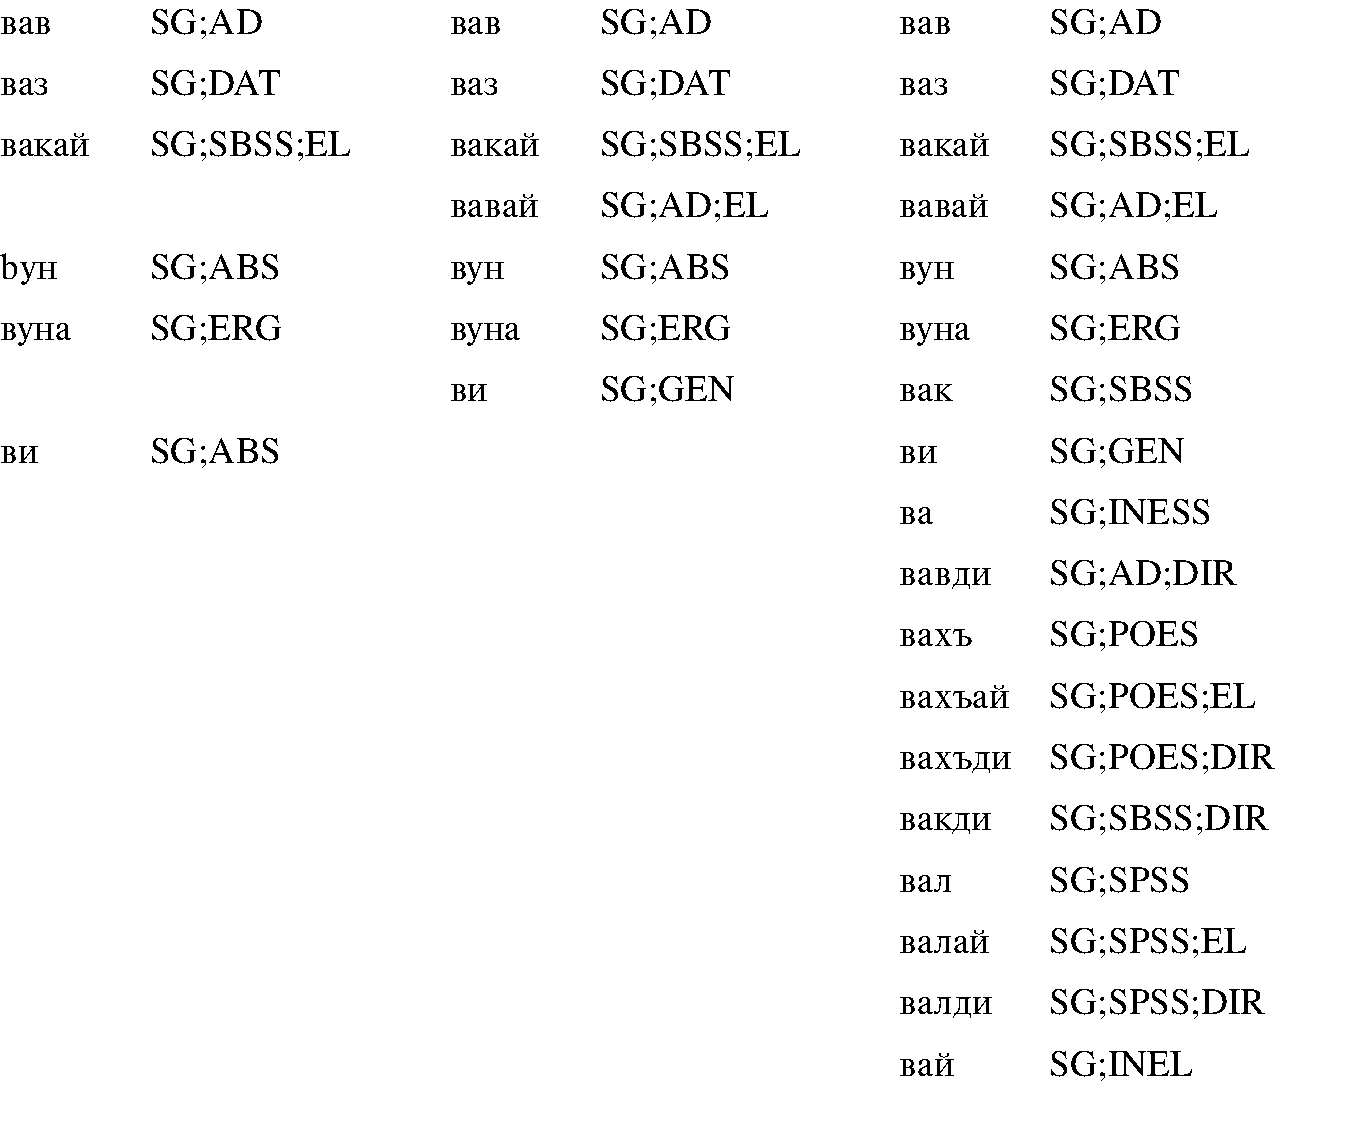
\includegraphics[width=15cm]{figs/LezgiParadigms.pdf}
    \caption[Noisy to Clean Paradigms]{Lezgi paradigms were automatically constructed from IGT (left column) which have typos, incorrect glosses, and wrongly clustered paradigms. Domain experts ``cleaned'' the automatically extracted paradigms (middle column). These can be compared with the published description (right column) which includes several forms that are rarely used in modern spoken Lezgi.}
    \label{fig:cleaning}
\end{figure}

\paragraph{Step 2: Preparing reinflection data.}
The typical morphological reinflection data is in tuple format of \texttt{(source form, target form, target features)}. The paradigm data is converted into this format in preparation for reinflection. Table \ref{tab:IGT2Pdata} presents the data sizes.\footnote{Inflection data available at: \url{https://github.com/LINGuistLIU/IGT}} 

For each language, the validation and test sets are prepared by using the expert-cleaned data language in the following way: If the paradigm has more than one form, pick a random form as the source form and select the remaining forms in the paradigm with a probability of 0.3 to be ``unknown'', i.e., to be predicted from the first form. Half of the ``unknown'' data transformed in this way is used for validation and the other half for testing. The validation and test sets for each language are shared across all the experiments conducted for that language.

To create training data from both noisy and clean paradigms, each inflected form is matched with its own morphosyntactic features and mapped to itself. Paradigms with a single entry have only this self-to-self mapping. If a paradigm has more than one form, all possible pairs of inflected forms plus morphosyntactic features within each paradigm are generated, excluding those that are part of testing or validation set, i.e., ``unknown''.
 

\paragraph{Step 3: Reinflection models and experimental setup.}
This experiment compares two state-of-the-art models for morphological reinflection, the Transformer model for character-level transduction \citep{wu2020applying} and the LSTM sequence-to-sequence model with exact hard monotonic attention for character-level transduction \citep{wu-cotterell-2019-exact}. For all the models, the implementation of the SIGMORPHON 2020 shared task 0 baseline was used \citep{vylomova2020sigmorphon},\footnote{\url{https://github.com/shijie-wu/neural-transducer/tree/f1c89f490293f6a89380090bf4d6573f4bfca76f}} and the hyperparameters for this study are the same as the shared task baseline.

After paradigms are extracted and preprocessed, two experiments were conducted to generate ``unknown'' inflected forms. Those experiments were then expanded by two data augmentation techniques. First, all unannotated/uninflected words from the IGT data are added to the training data. When tokens that were either unannotated or uninflected are added, they are self-mapped as source and target forms (exactly as with single-entry paradigms), and their morphosyntactic features are annotated with a special tag: \texttt{XXXX}.  Second, the training data was augmented by generating 10,000 artificial instances with the implementation in the SIGMORPHON 2020 shared task 0 baseline of the data hallucination method proposed by \citet{anastasopoulos-neubig-2019-pushing}. Finally, both additions are combined. These augmentations are intended to overcome data scarcity. 


\section{Results}
\label{sec:IGT2Presults}

All models and techniques were tested on the same held-out set chosen randomly from multi-entry paradigms in each language. Results were compared when trained on the noisy paradigms and on the expertly cleaned paradigms. The results are displayed in Table \ref{tab:IGT2Presults}. With few exceptions, it shows that the limited involvement of experts cleaning the data improves results over training on the noisy data. Also, the best Transformer results surpassed the best LSTM with hard monotonic attention. The primary exception to both these statements is the Alas [btz] results. This perhaps because it is the smallest corpus, roughly half or two-thirds the size of the next largest corpus (Lezgi). Alas also has the poorest results by far of all the languages.
Comparing results from augmenting the data by artificial and uninflected/unannotated tokens gave varied results. The factors affecting these varied results are unclear although the consistency of the noise and the extent of cleaning may be factors. 


\begin{table}[!tb]
    \centering
    \setlength{\tabcolsep}{8.pt}
    \begin{tabular}{l|cccc|cccc}
      \textbf{} & \textbf{T} & \textbf{+aug} & \textbf{+uninfl} & \textbf{+both} & \textbf{mono} &  \textbf{+aug} &
      \textbf{+uninfl} &
      \textbf{+both} \\ 
       \hline
      arp clean & \textbf{62.08} & 61.39 & 61.58          & 60.78 & 15.93 & 15.75 & 15.58 & 15.94 \\
      arp noisy & 57.77          & 57.64 & \textit{58.04} & 57.51 & 14.51 & 14.64 & 14.52 & 14.69 \\
      % diff:   & 4.31           & 3.75  & 3.54           & 3.27 
      % Relatively slight differences. This and ddo were probably most complete and polished data. In fact, can hardly be called field data. Also, the largest ones. The bigger differences in the other datasets show how important this technique is when working with actual field data. It may indicate a point of reduced returns on cleaning time.  
      \hline
      btz clean & 7.69 & 3.85 & 1.92 & 1.92 & 1.92 & 5.77 & 1.92 & 1.92  \\
      btz noisy & 9.62 & 9.62 & 13.46 & 3.85 & 5.77 & 13.46 & 1.92 & \textbf{17.31}  \\
      % Measured by paradigms roughly same amount of data as Lezgi, but significantly fewer total tokens. Train data has almost half in clean data and roughly 1/4 of the Lezgi data. Higher proportion of single-entry forms (to tokens - btz clean: 45%, btz noisy: 36%; lez clean: 37%, lez noisy: 32%. to train - 49%, 26; 37%, 15%). More unannotated tokens in comparison to noisy train data. Combined with less data period. So could this mean less repeated roots in paradigms, fewer repeated inflected forms. But probably mostly due to difference in language structure. It is not clear what. Presumably, there are more inflected POS in BTZ and therefore more variability in training data.
      \hline
      ddo clean & 65.38 & \textbf{66.53} & 65.19 & 65.42          & 59.9 & 60.87 & 59.53 & 60.64  \\
      ddo noisy & 63.54 & 63.95          & 62.89 & \textit{64.04} & 59.12 & 58.66 & 57.87 & 57.97 \\
      %diff:    & 1.84  & 2.58           & 2.30  & 1.48       
      % Smallest differences. Is the slight difference due to the polished state of the data? Or the lack of knowledge of expert?
      \hline
      lez clean & 46.59          & 32.95 & 46.59 & \textbf{48.86} & 32.95 & 35.23 & 31.82 & 31.82 \\
      lez noisy & \textit{35.23} & 29.55 & 32.95 & 27.27          & 30.68 & 28.41 & 20.45 & 31.82 \\
      % diff:   & 11.36          & 3.40  & 13.64 & 21.59
      % Biggest range of differences. So weird that both augmentation techniques got worst results in noisy data but best in clean data.
      \hline
      mni clean & 30.63 & 30.87         & 31.81 & \textbf{32.04} & 23.24 & 25.7 & 21.95 & 24.77 \\
      mni noisy & 21.48 & \textit{22.3} & 21.60 & 21.83          & 18.78 & 18.31 & 19.37 & 20.31 \\
      % def:    & 9.15  & 8.57          & 10.21 & 10.21
      % Biggest consistent differences. Most changes in cleaned data. 
      \hline
      ntu clean & \textbf{53.18} & 46.82 & 49.15 & 48.52          & 29.66 & 33.9 & 28.18 & 33.05 \\
      ntu noisy & 36.86          & 45.55 & 45.34 & \textit{45.76} & 31.99 & 33.69 & 31.78 & 30.93 \\
      % def:    & 16.32          & 1.27  & 3.81  & 2.76
      % Why did the data cleaning in ntu make such a significant difference but not with augmentation? Note that augmented data is not cleaned of course. Most cleaning time spent here. This and Arapaho were cleaned by highly expert linguists who spent years on the language. Others were cleaned by linguists who had spent only a few years, in some cases several months, working on the language. 
    \end{tabular}
    \caption[IGT2P Results]{Accuracy percentages of reinflection task from the Transformer (T) and the LSTM seq2seq model with exact hard monotonic attention (mono) with/out artificial data augmentation (+aug), unannotated/uninflected word forms (+uninfl) and both together. Boldface indicates best result; italics indicate best result on noisy paradigms.}
    \label{tab:IGT2Presults}
\end{table}

There is no clear correlation between accuracy and the total number of annotated tokens or training paradigms (see Tables \ref{tab:dissdata} and \ref{tab:IGT2Pdata}). Tsez and Arapaho [arp] achieved over 60\% accuracy and these languages do have more training data (35K and 283K triples, respectively) than the others (less than 10K). However, even though Arapaho has considerably more training data, its accuracy is lower than Tsez. A slight correlation between accuracy and amount of multi-entry paradigms does exist. Languages with a higher proportion of multi-entry paradigms tend to have better results. Fewer single-entry paradigms may indicate more complete paradigm information.
%because single-entry paradigms are missing forms, and this may cause inconsistency during inflection inference. 

Any correlation between results and linguistic factors such as language family or morphological type is uncertain because of the limited number of languages. Tsez [ddo] gave best results overall. This could be due to its limited allomorphy and very regular inflection which may explain why Lezgi [lez], which is closely related to Tsez, performs better than languages with more data. Arapaho's poorer performance could be due to its polysynthetic morphology \citep{cowell_arapaho_2008} which is more complex than the fairly straightforward agglutination in Tsez \citep{job_tsez_1994} and Lezgi \citep{haspelmath_grammar_1993}. The models do seem less sensitive to recognizing the word structure in Arapaho. When the first part of a stem is incidentally the same as a common inflectional affix, the stem is often generated incorrectly. This result in a misspelled stem. 

%On the other hand, Arapaho [arp] has relatively clean annotations but its morphological patterns are much more complex. %However,  this is undoubtedly due to the varying quality of IGT annotations and to the differing morphological structures of the languages. 

The factor that seems most clearly correlated with accuracy is the consistency and thoroughness of IGT annotations. The Arapaho, Tsez, and  Nat\"ugu [ntu] corpora were noticeably more complete (i.e., most morphemes were glossed) and consistent. This probably explains why Tsez not only had the best results but also showed the smallest improvements after cleaning. Interestingly, augmentation techniques helped these languages the least (only artificial data augmentation helped Tsez slightly). It seems, therefore, that data augmentation is most helpful when original manual annotations are most consistent or complete. 

% error analysis
As might be expected with limited data, errors were most common with irregular or rare forms. For example, the best performing model incorrectly inflected many Lezgi pronouns which have an inflection pattern identical to nouns except for an unpredictable change in the stem vowel. Perhaps related to this, the model also misidentified some epenthetic vowels in several Lezgi nouns. Another interesting pattern involved unique Nakh-Daghestanian (Tsez and Lezgi) case-stacking, where nominal affixes concatenate, rather than substitute each other, to form several peripheral cases such as \textsc{genitive} (cf. (\ref{ex:Lezgi3})). The more common affixes in the concatenated strings were often generated correctly but the less common concatenated affixes were not. Allomorphy also causes difficulty. Models tend to generate the right form less often when multiple forms are possible. This seems particularly true for Arapaho which also has many similar forms that mark similar, but not identical, information. For example, in Arapaho similar agreement affixes on verbs were often ``confused'', such as -oo `\textsc{obj} (of transitive verb with animate object)', -o' `\textsc{1.sg.actor/3.sg.undergoer} (of transitive verb with animate object)', and -' `\textsc{3.sg.actor} (of intransitive verb with inanimate subject)'. All these affixes had a low accuracy of prediction by the model. On the other hand, models learned regular inflectional patterns well enough to correctly inflect forms to the extent that where the expert had left misspellings of that form in the cleaned data, the model ``corrected" it.

%expert cleaning
Finally, we clearly see expert cleaning improved performance across the board (with two negligible exceptions for Tsez and Lezgi on the hard monotonic attention model). Experts were asked to spend no more than six hours and actually spent up to seven but as little as two hours on each language. This indicates that expert labor is well worth its cost. 


\section{Conclusion}

We proposed a new morphological generation task called IGT2P, which aims to learn inflectional paradigmatic patterns from interlinear gloss texts (IGT) produced in linguistics fieldwork. We experimented with neural models that have been used for morphological reinflection and new preprocessing steps as baselines for the task. Our experiments show that IGT2P is a promising method for creating new morphological resources in a wide range of low-resource languages. 

With sufficient IGT annotations, IGT2P obtains reasonable performance from noisy data. 
We investigated the effect of manual cleaning on model performance and showed that even limited cleaning effort (2-7 hours) drastically improves results. The inherent noisiness in IGT and other linguistic field data can be overcome with limited input from domain experts. This is a significant contribution considering the extensive effort---on the order of months and years---to produce the curated structured data normally used to train NLP models. 
In languages with the noisiest data the model's performance is improved even further by data augmentation techniques.

There is room for future improvement. Better techniques for further cleaning might be useful since accuracy seems to be closely related to data quality. However, at some point more cleaning will return less improvement. Upper bounds could be established by comparing results on languages with gold standard inflection tables, although polysynthetic languages like Arapaho would make this difficult since their tables do not always include noun incorporation. Better use of experts' time might involve identification of lemmata that could be used to train a lemma-to-form model, rather than the form-to-form mapping used here. Another approach would be to compare improvements between manual-only cleaning and cleaning done by a linguist working with someone who can write scripts to automatically correct repeated patterns of noise. 

IGT2P also has implications for the documentation of endangered languages and addressing digital inequity of speakers of marginalized languages. It could be integrated into linguists’ workflow in order to improve the study of inflection and increase IGT data. For example, the generated inflected forms could be used for automated glossing of raw text. IGT2P could speed the discovery and description of a language's entire morphological structure. An elicitation step with native speakers could be added to strategically augment data. This would integrate well with linguists’ workflow. IGT2P results could serve to prompt speakers for forms that are rare in natural speech. It might also be integrated into linguistic software such as FLEx.